\chapter{Hardware}

\section{Controller: Microchip PIC32MX695F512H}
The core of the system is the powerful Microchip PIC32MX695F512H controller, which directly interfaces with each of the system's peripherals. This controller was chosen due to the high processing speed, low cost, and abundant peripherals. It operates at 3.3V with an instruction clock of 80MHz, referenced to an 8MHz crystal for improved stability with the extreme temperature fluctuations provided by the amplifiers. The controller is based on a MIPS32 M4K 32-bit core, featuring a 5-stage pipeline, 512kB of flash program memory (with an additional 12kB available for a bootloader), and 128kB of RAM. The chip uses a a 64-pin TQFP package.
\subsection{Hardware Peripheral Support}
The PIC32MX695F512H Its abundant hardware peripherals include:
\begin{itemize}
\item 4 I\superscript{2}C channels
\item 3 SPI channels
\item 16 channel 10-bit ADC
\item 2 analog comparators
\item 10/100Mbit ethernet controller
\item USB 2.0 transciever with On-The-Go (OTG) and full-speed capabilities
\item 6 UART channels
\item 5 16-bit timers
\item 5 Output Compare modules
\item 5 Input Capture modules
\item Up to 53 general purpose I/Os, many of which are 5V tolerant. 
\end{itemize}
\begin{figure}[H]
	\centering
	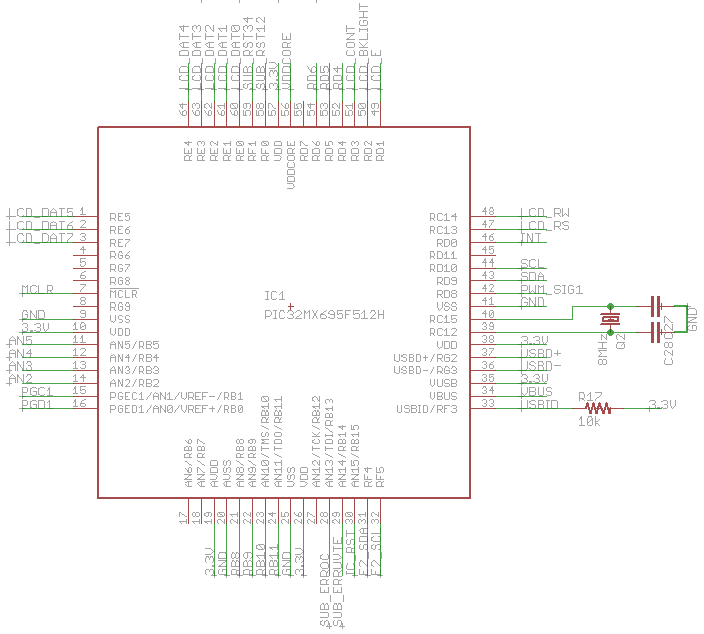
\includegraphics[width=4in]{schem-pic32}
	\caption[Schematic -- Microcontroller]%
	{Schematic of the PIC32MX695F512H and surrounding connectivity}
\end{figure}
The following communications peripherals are used in our system:
\subsubsection*{I\superscript{2}C}
I\superscript{2}C (\textbf{I}nter-\textbf{I}ntegrated \textbf{C}ircuit) is a bi-directional, synchronous, serial bus which requires minimal connectivity and can have any number of masters or slaves. Only two signalling wires are required: SDA (\textbf{S}erial \textbf{DA}ta) and SCL (\textbf{S}erial \textbf{CL}ock.) Since, unlike with SPI, there is no \textit{select} line, slave selection is done by prefixing all operations with the address of the intended slave. The I\superscript{2}C bus is used primarily as a messaging bus due to its minial connectivity requirements and low maximum clock rate, which is usually 100 or 400kHz, making it ill suited for applications requiring high data throughput. All of our peripherals operate only as slaves and the controller acts only as a master.
\subsubsection{10-bit ADC}
The 10-bit \textbf{S}uccessive \textbf{A}pproximation \textbf{R}egister (SAR) \textbf{A}nalog-to-\textbf{D}igital \textbf{C}onverter (ADC) has a 16-input analog multiplexer and can sample values from 0V to 3.3V ($V_{DD}$) at up to 1MHz.
\subsubsection{USB Transciever}
The USB transciever is not used in the system for any essential function. It may be used for programming if there is any trouble with the PICkit2 programmer. The Microchip USB library provides facilities to implement the USB \textbf{C}ommunications \textbf{D}evice \textbf{C}lass (CDC) for simple messaging with a PC for easy debugging.
\subsubsection{General Purpose Input/Outputs}
The selectably bidirectional I/O banks are robust, offering a number of features that are configurable on a per-pin basis:
\begin{itemize}
\item Weak pull-ups for inputs to eliminate the need for external resistors
\item Generate interrupt on selectable edge
\item Select complementary or open-drain to allow driving voltages higher than $V_{DD}$
\end{itemize}
\subsubsection{Output Compare}
The output compare modules compare the value of a timer to one or two fixed values and with output connected to an I/O pin. For our applications, this allows the ability to output a PWM signal using a timer that is continuously looping past a single comparison value.
\subsubsection{Input Capture}
Input capture allows timer values to be captured upon external events. This is useful in a wide array of applications where pulses need to be detected and characterized. Our system uses it to take input from a PWM signal.

\subsection{Programming}
Microchip offers a free C compiler, MPLAB C32, for educational use. Compiled code can be loaded to the chip using the \textbf{I}n-\textbf{C}ircuit \textbf{S}erial \textbf{P}rogramming (ICSP) header on the board and a PICKit2, which is a small USB programming device. Programming may also be done directly over USB to the controller by incorporating Microchip's USB bootloader into our code.

\section{Amplifier A -- Cirrus CS4245}
The Cirrus CS4245 is a 4-channel Class-D (digital) amplifier with an integrated stereo ADC and audio signal processing capabilities.

\subsection{ADC}
The 24-bit 48kHz SAR ADC connects to the output of the input bandpass filter. This bandpass filter eliminates higher frequency noise as well as isolating the $V_{DD}/2$ DC bias applied internally to center the input in the ADC range. This high-frequency noise is particularly dangerous, as it can include high voltage spikes that can damage the ADC. Additionally, it is detrimental to audio fidelity to sample at above the Nyquist freqency ($f_s/2 = 24$kHz), as components above that frequency will appear as if they were folded over the Nyquist frequency.
\begin{figure}[H]
	\centering
	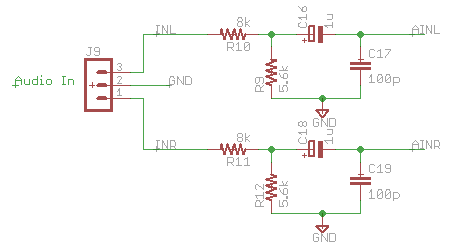
\includegraphics[width=4in]{schem-input}
	\caption[Schematic -- Analog Input Filtering]%
	{Schematic of the amplifier input filters}
\end{figure}
To operate the ADC, the system uses a 24.576MHz ($48$kHZ$*512$) crystal for its clock source.

\subsection{Output}
The output of a digital amplifier is a PWM signal which must be filtered through an analog network to reproduce the input signal. The frequency of this signal is configurable on the amplifier (to reduce AM interference) and is normally in the range of 300 to 400kHz. Logic-level outputs are also provided to allow the signals to be passed to another amplifier. The CS4525 can be configured to mix a subwoofer channel as well, using one of these logic-level ouputs.
\begin{figure}[H]
	\centering
	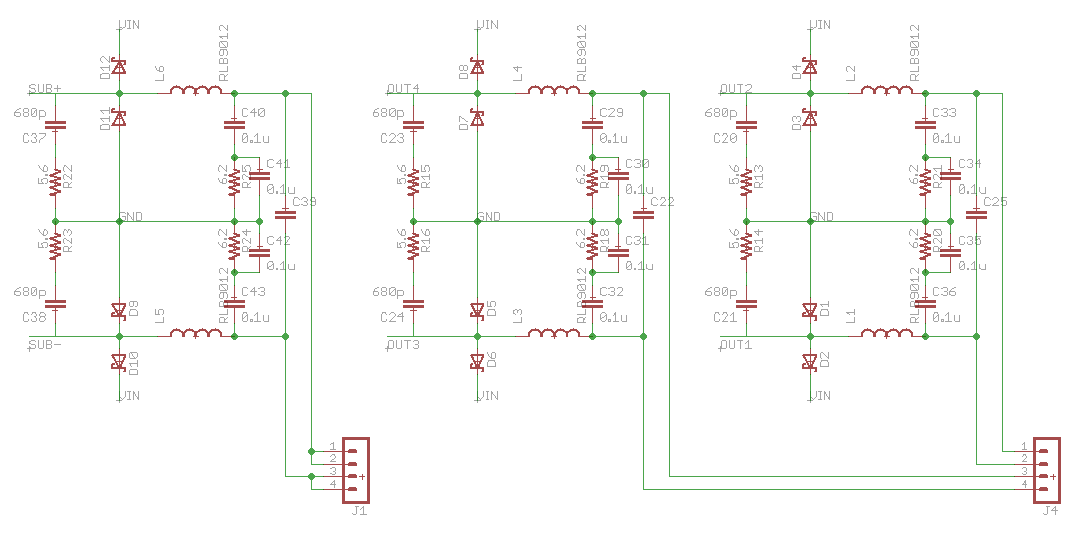
\includegraphics[width=6.5in]{schem-output}
	\caption[Schematic -- Amplifier Output Filters]%
	{Schematic of the output filters for the subwoofer, left, and right channels}
\end{figure}
Though there are 4 single-ended outputs, we use them in a stereo \textbf{B}ridge-\textbf{T}ied \textbf{L}oad (BTL, also known as \textit{H-Bridge}) configuration which uses two single-ended outputs, one inverted from the other, for each channel. The difference between each pair is taken as the output for each channel, providing a maximum voltage swing of $2V_{IN}$. For a fixed load impedance, this is an 4-fold increase in power over a single-ended configuration.
\subsection{Communications}
The CS4525 is controlled over I\superscript{2}C in addition to asynchronous interrupt (output) and reset (input) lines. The LSB of the slave address of the device is configured in hardware by tying a pin to either $V_{CC}$ or ground. The amplifier cannot report errors solely using I\superscript{2}C, since it is required that the master initialize each communication. The asynchronous interrupt line is therefore used to signal to the controller that it must read the \textit{Interrupt Status} register in order to determine the nature of the error. The accepted logic level of the amplifier is configurable and set to 3.3V in our case.
\subsection{DSP}
\label{sec:dsp}
The onboard DSP of the CS4525 provides a number of built-in effects that can be individually selected and controlled:
\begin{description}
\item[Equalizer] \hfill \\
Adjustable gain for configurable frequency ranges corresponding to \emph{Bass}, \emph{Mid-range}, and \emph{Treble}. 
\item[Dynamic Loudness Compensation] \hfill \\
The input volume is scaled to maintain an acceptable short-time average power. This has the effect of normalizing volume levels to improve audibility of material.
\item[Thermal Foldback] \hfill \\
In the case of an unacceptable increase in temperature, the amplifier can automatically reduce its volume incrementally until a safe temerature is reached. This should offer the protection necessary to avoid the need for shutdown due to a thermal error condition.
\item[BiQuad Filter] \hfill \\
A standard biquad filter is available with programmable filter coefficients to implement a generic, user-designed filter.
\end{description}

\subsection{Power}
As a class-D amplifier, the CS4525 is very efficient, delivering approximately 90\% of its consumed power to the loads. It uses a compact 48-pin QFN package with an additional thermal pad on the underside of the chip for heat transfer. The chip is designed to operate without a heatsink, therefore imposing design restrictions on the circuit board to maximize distribution and dissipation of heat.
\begin{figure}[H]
	\centering
	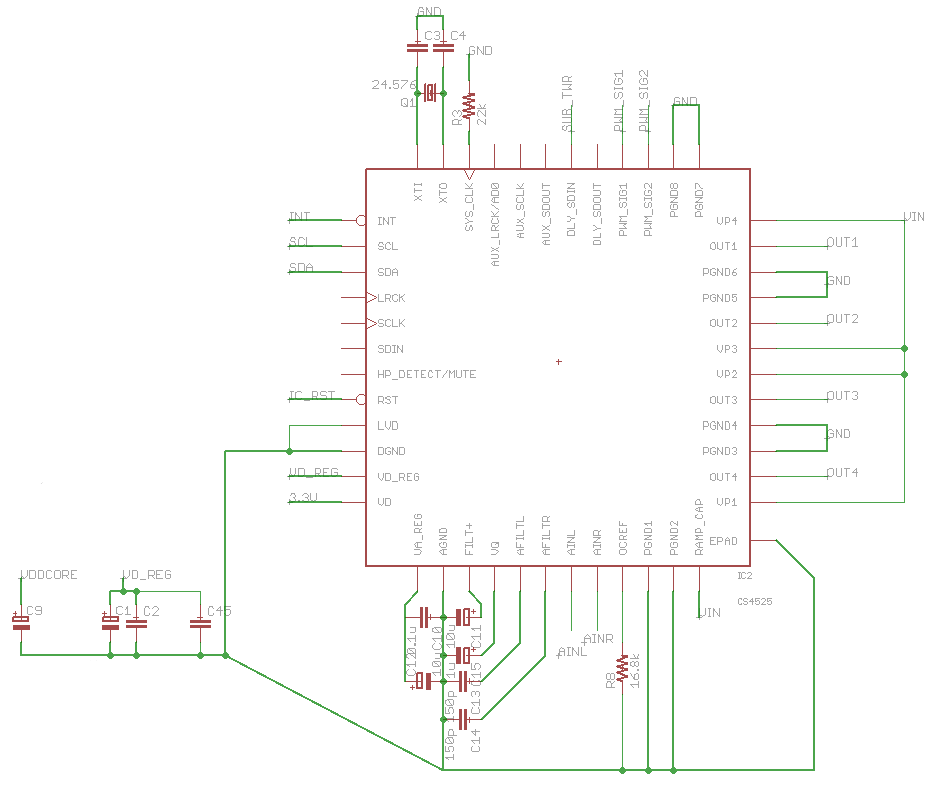
\includegraphics[width=5in]{schem-cs4525}
	\caption[Schematic -- CS4525 Amplifier]%
	{Schematic of the CS4525 and its connectivity}
\end{figure}


\section{Amplifier B -- Cirrus CS4412}
The Cirrus CS4412 contains the same amplifier circuitry as the CS4525 but without the ADC and signal processing features. It is therefore well suited as a peripheral to the CS4525, amplifying an additional channel. It uses a remixed, processed, logic-level signal from the CS4525 for input and is connected in a mono BTL configuration to a lower impedance subwoofer. As this amplifier is not capable of any bus communications, any errors are caught by the interrupts on the PIC32. For thermal conditions that would not warrant an error but do require notification of the amplifier for the application of thermal foldback, there is an additional line to notify the CS4525 of this state. 
\begin{figure}[H]
	\centering
	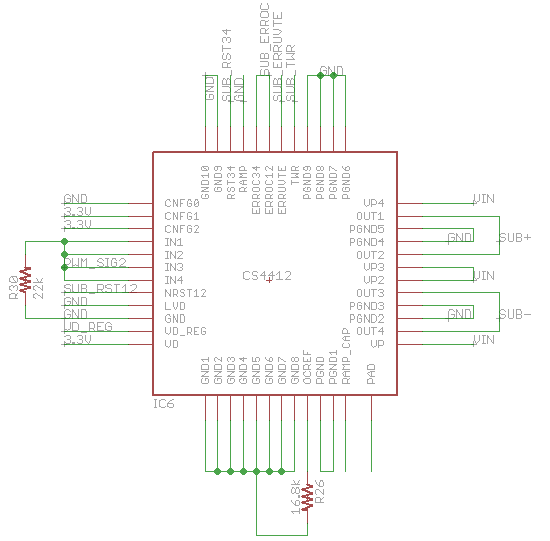
\includegraphics[width=4in]{schem-cs4412}
	\caption[Schematic -- Cirrus CS4412]%
	{Schematic of the CS4412 amplifier and its connectivity}
\end{figure}
Like the CS4525, it can handle up to 30W but is driving only a single load. The CS4412 also comes in a 48-pin QFN with a similar thermal pad on the bottom, imposing the same PCB layout restrictions.

\section{EEPROM -- Microchip 24FC1025}
\label{sec:eeprom}
The 24FC1025 is a common I\superscript{2}C EEPROM addressing 1024kB of data and offering a minimum of 1 million write cycles and 200 years of data retention. As the microcontroller has only flash (which supports far fewer write cycles) available as non-volatile memory, the system uses the EEPROM for long term storage of settings. As there are an excess of I\superscript{2}C channels, the system uses a second channel rather than sharing with the CS4525. The chip comes in a n 8-pin PDIP and happily operates at 3.3V. 
\begin{figure}[H]
	\centering
	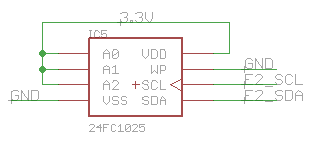
\includegraphics[width=3in]{schem-eeprom}
	\caption[Schematic -- Microchip 24FC12025]%
	{Schematic of the Microchip 24FC1025 EEPROM and its connectivity}
\end{figure}


\section{LCD -- Hitachi HD44780}
\label{sec:lcd}
The 16x2 blue-backlit character LCD employs the industry-standard protocol of the Hitachi HD44780 controller. The specifications for the protocol allow for either a 4-bit or 8-bit wide data bus, and due to the large number of unused pins, we have opted for the faster 8-bit bus. The 16-pin HD44780 header includes these 8 data pins as well as \emph{Enable}, \emph{Read/Write Select}, and \emph{Register Select}. Additionally, there is a connection for power to the backlight as well as a contrast adjustment pin usually controlled with a voltage divider. These are both instead controlled by PWM, so as to be software-adjustable. As the LCD is natively 5V, the pins on the controller must be used as open-drain to allow access to the full 5V of the LCD. The LCD is accepting of the 3.3V input provided by the microcontroller. Additionally, the microcontroller pins used for the data lines from the LCD are tolerant of the 5V from the LCD.

\section{Buttons}
\label{sec:buttons}
Capacitive buttons are implemented using the PIC32MX695F512H's ADC, which is used periodically for each of 4 buttons: \emph{Menu/Select}, \emph{Exit}, \emph{Home}, and \emph{Mute}. Capacitive buttons use the variations in capacitance of a conductor caused by the user's finger touching the button. To do this with an ADC, the ADC is first connected to $V_{DD}$ by the multiplexer to fully charge the sample-and-hold capacitor in the ADC. The pin for the button is set as a digital output to ground to ensure that it holds no charge. The pin is then selected as an analog input, connecting the uncharged capacitance of the switch to the sample and hold capacitor in the ADC. This has the effect of a capacitive voltage divider, presenting an approximate relative value of the capacitance of the switch. The system tracks those values over time, watching for variations from an average of recent samples. 

\section{Continuous Rotary Switch}
\label{sec:rotary}
The rotary switch uses a 12-position make-before-break rotary switch and 3 general purpose I/Os to detect each transition. The selector pin of the rotary switch is tied to ground, with 3 input pins assigned in cycles around the switch with weak pull-ups enabled. At any rest state, there will be one pin pulled to ground by the selector. In the transition state in either direction, one of the adjacent pins will throw an interrupt on the falling edge as it is pulled to ground by the selector. Only when the previous pin becomes disconnected will the switch operation be recognized as complete. Since the total number of positions is a multiple of 3, the order of the pins on the switch will be repeated 4 times.

\section{Power Regulation}
The board requires 3 stable voltage levels to operate:
\begin{description}
\item[3.3V ($V_{DD}$)] \hfill \\
3.3V is considered the primary logic-level voltage for the system, powering the amplifier logic, the microcontroller, and the EEPROM. This level is provided by an adjustable LM317 positive regulator with appropriate component values to provide 3.3V. This regulator can deliver up to 1.5A, which is well above the maximum power draw of dependent components. 
\item[5V] \hfill \\
5V is required for the LCD and is provided by an LM78L05 5V positive low-dropout regulator. This regulator is able to provide up to 100mA, well exceeding the maximum power draw of the LCD.
\item[$V_{IN}$] \hfill \\
This is the level provided by the power supply of approximately 18V. This powers the amplifiers and the regulators for other voltage levels. It must safely handle an estimated 80W at the very minimum.
\end{description}

\begin{figure}[H]
	\centering
	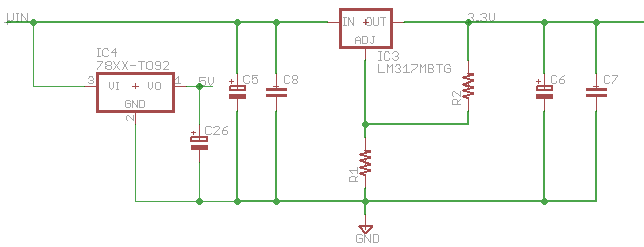
\includegraphics[width=4in]{schem-power}
	\caption[Power Regulation]%
	{Schematic of the power regulator circuitry}
\end{figure}

\section{Circuit Board}
\begin{figure}[H]
	\centering
	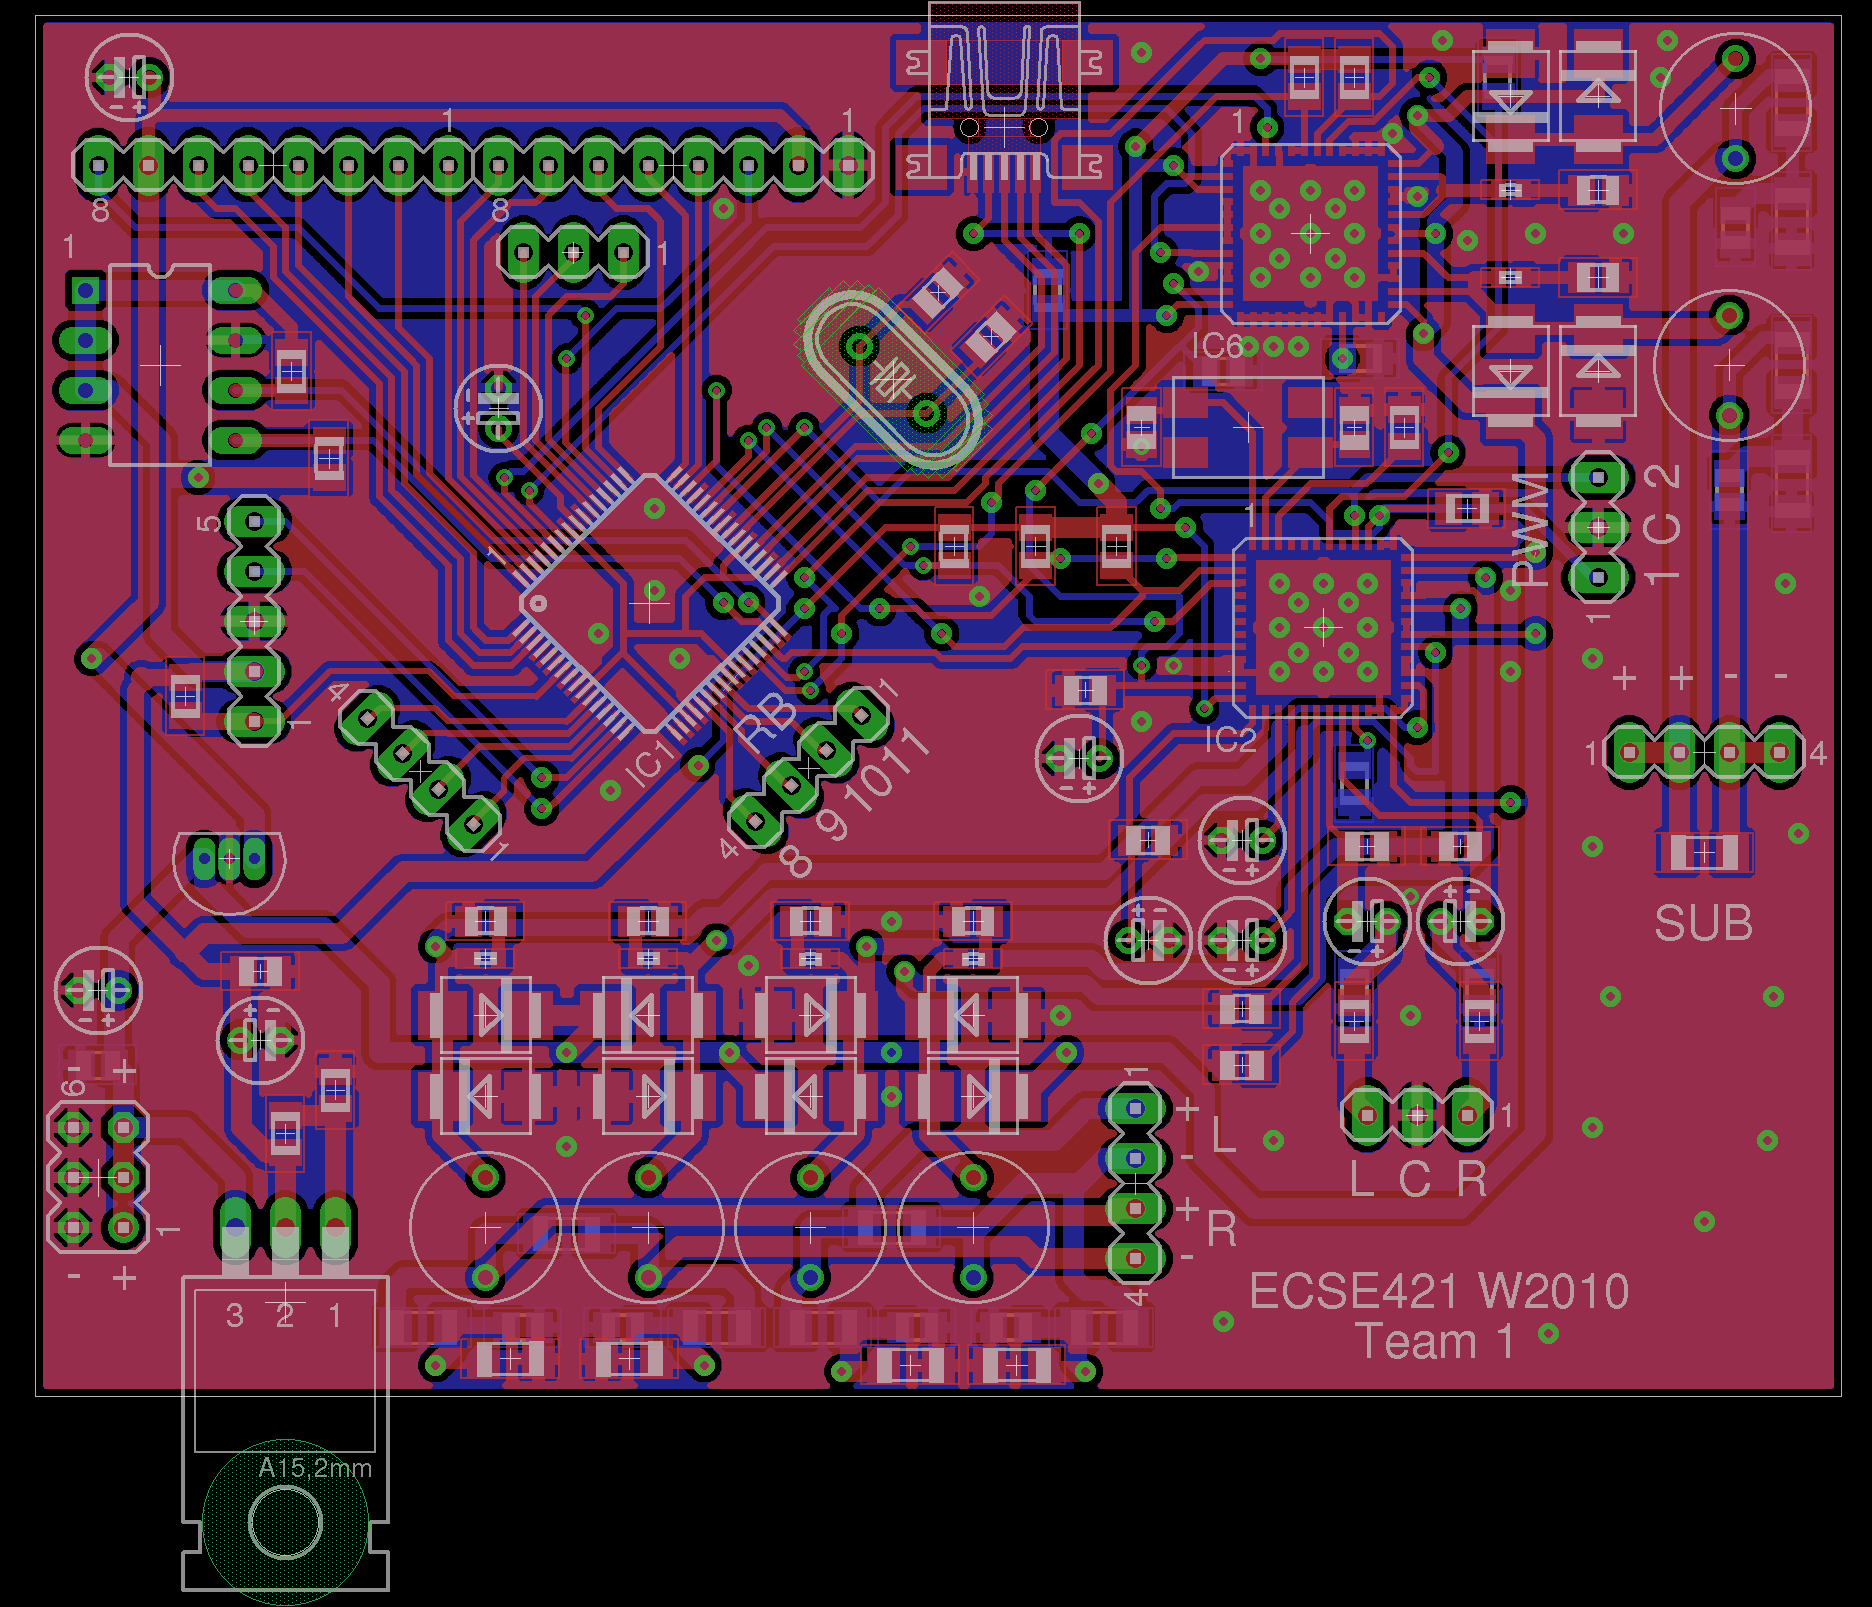
\includegraphics[scale=1.8, angle=270]{board}
	\caption[PCB Layout]%
	{Printed circuit board layout}
\end{figure}
